\documentclass[UTF8]{article}
\usepackage{amsmath}
\usepackage{ctex}
\usepackage{geometry}
\usepackage{graphicx}
\usepackage{float}
\usepackage{array}
\usepackage{longtable}

\DeclareGraphicsExtensions{.eps,.ps,.jpg,.bmp}
\geometry{top=3.18cm,bottom=3.18cm}
\usepackage{mhchem}
\begin{document}
	\title{\heiti 本研中期成果证明材料}
	\author{\songti 刘畅\\北京大学物理学院天文系}
	\date{}
	\maketitle
\begin{fangsong}
\section{复现无X射线环境下分子云中的化学演化过程}
复现 Wakelam \& Herbst 2008 的 Fig.3 和 Fig.4 中,不考虑多环芳烃(PAH)的 EA1(灰色实线), EA2(灰色虚线), EA3 (灰色点虚线)模型下各物质的丰度随时间的演化。
\begin{figure}[htbp]
	\centering
	\begin{minipage}[t]{0.50\textwidth}
		\centering
		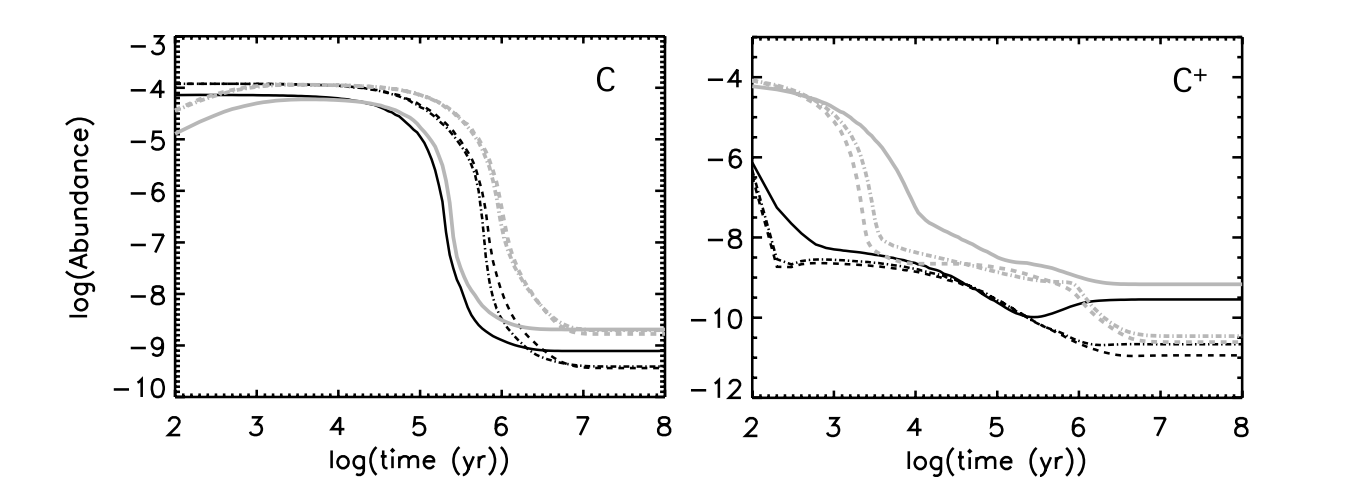
\includegraphics[width=7cm]{Wakelam1.png}
		\caption{Wakelam \& Herbst 2008 Fig.3}
	\end{minipage}
	\begin{minipage}[t]{0.49\textwidth}
		\centering
		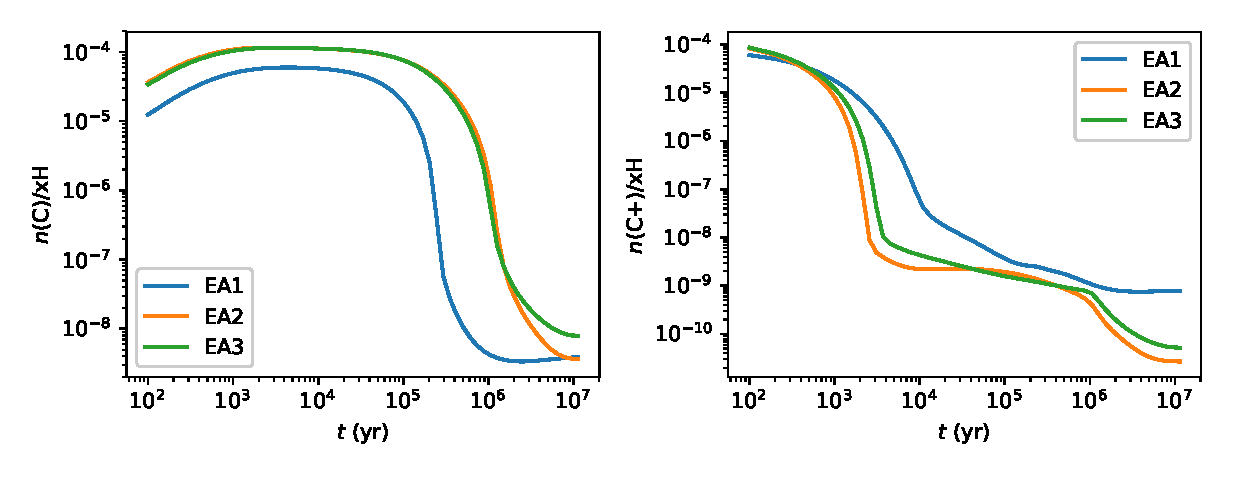
\includegraphics[width=6.5cm]{1.eps}
		\caption{复现三种模型中$\ce{C,C+}$的演化}
	\end{minipage}
\end{figure}

\begin{figure}[htbp]
	\centering
	\begin{minipage}[t]{0.49\textwidth}
		\centering
		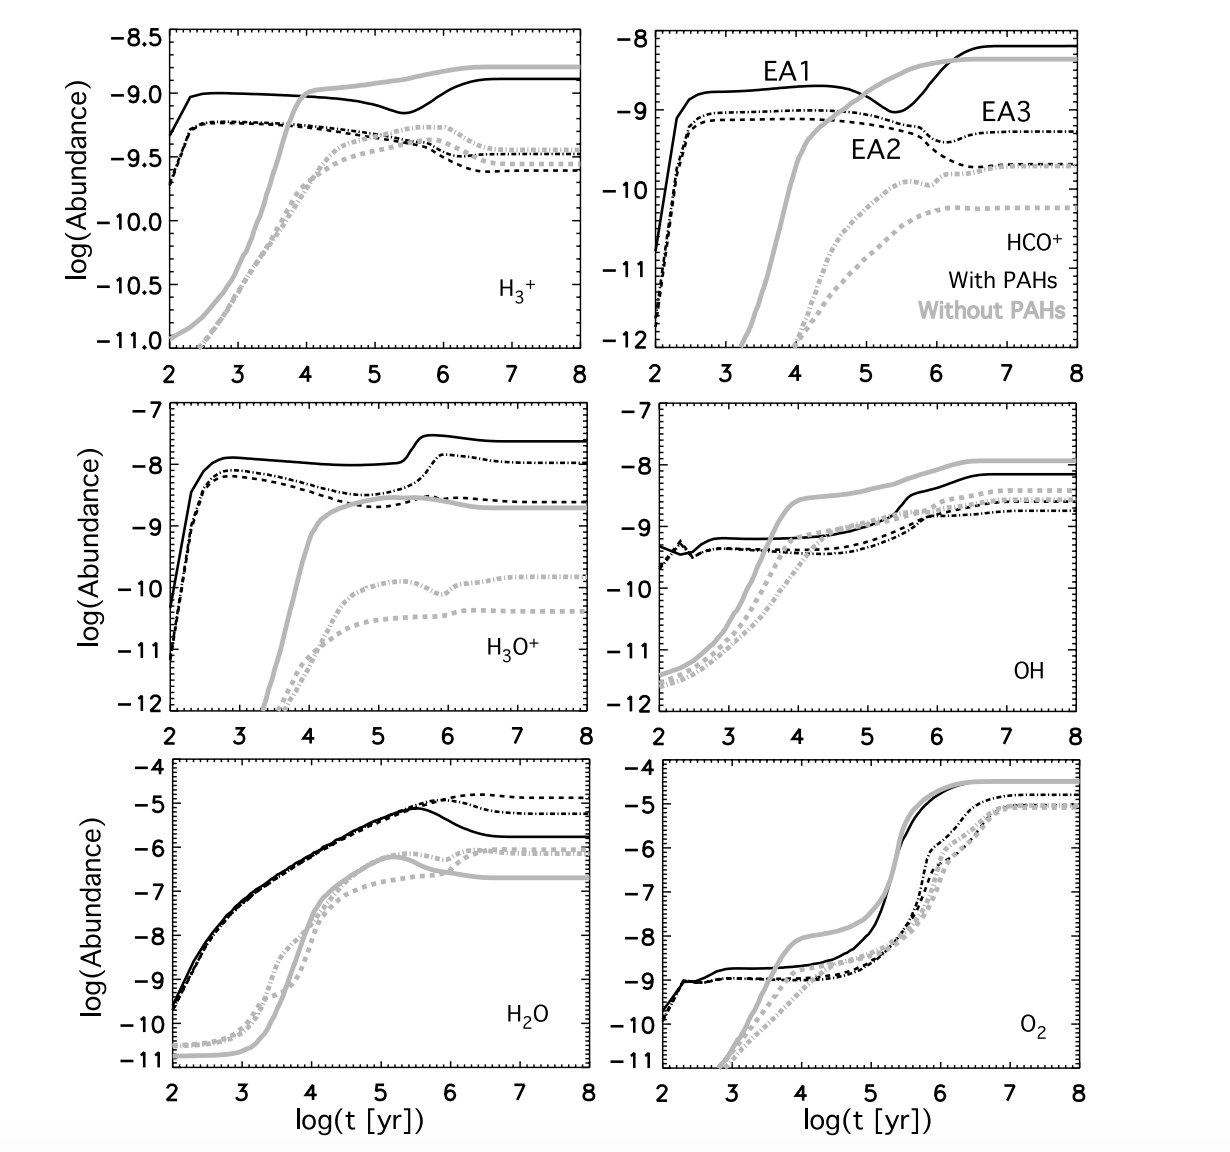
\includegraphics[width=7.5cm]{Wakelam2.png}
		\caption{Wakelam \& Herbst 2008 Fig.4}
	\end{minipage}
	\begin{minipage}[t]{0.49\textwidth}
		\centering
		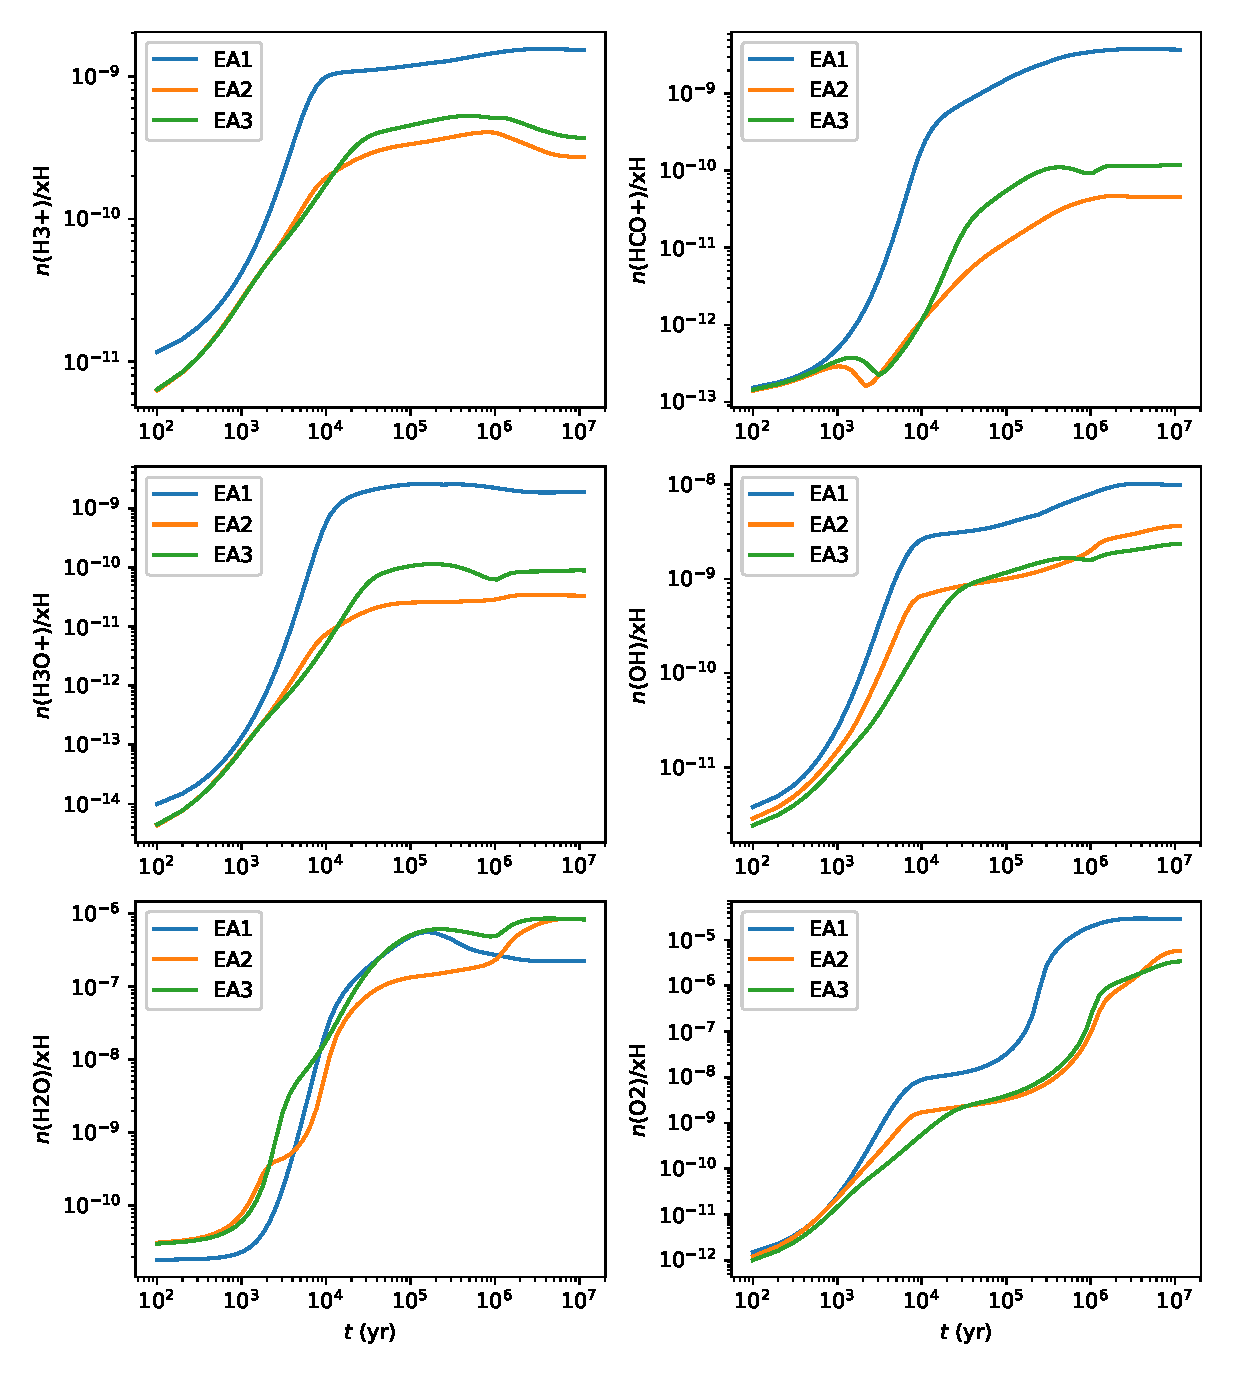
\includegraphics[width=6.5cm]{2.eps}
		\caption{复现三种模型中$\ce{H3+,HCO+}$, $\ce{H3O+,OH,H2O,O2}$的演化}
	\end{minipage}
\end{figure}

\section{银河系中心超大质量黑洞在离银心不同距离处的能谱、流量和引发的电离速率}
\section{复现X射线辐射下分子云中一些物质对电离率的响应程度}
复现 Krolik \& Kallman (1983) 中特定强度的宇宙射线和X射线下,一些物质的丰度对电离率的响应 
\end{fangsong}
\end{document}
